\chapter{Advanced SteamCAD Functions}\label{chap:chap3}
\special{pdf: out 1 << /Title (\thechapter. Advanced SteamCAD Functions) /Dest [ @thispage /FitH @ypos ] >>}

SteanCAD is especially designed to create high quality drawings with precise
dimensions at exact scale. Its main purpose is to prepare output for printing
or other publishing. To achieve this aim requires few more functions and
utilites. Let's look at the rest of the SteamCAD functionality in this
chapter.

\section{Setting Page Dimension, Drawing Scale and Defaults}\label{sec:settings}
\special{pdf: out 2 << /Title (\thesection. Setting Page Dimension, Drawing Scale and Defaults) /Dest [ @thispage /FitH @ypos ] >>}

As was said, SteamCAD output is primarily intended for presentations, that's why
each SteamCAD drawing must have a page defined. To do this, open the \textbf{File \lar{}
Properties} dialog. This dialog serves to set up all important values for the drawing
and should be invoked for each new file.

First you should select the page size from the combo box with predefined values.
Initially, A4 - A0 plus US Letter and US Legal paper sizes are available. But SteamCAD
is not restricted to those predefined paper sizes. You can add any paper size you
like into the DPapers.ini file. Let us remind you that this file should be copied
to your home folder, under hidden .SteamCAD subfolder on Linux systems and should
be in the folder with SteamCAD.exe on Windows systems. Open the file and examine its
structure. It is very simple, it contains list of semicolon separated values. Each
line of this file represents one paper size. The first value is the paper name, as
it appears in the combo box. The second value is the abbreviation of units used to
specify the page dimension. The last two values are actually the width and height
of the paper. The width should be less than the height, thus the paper is considered
to be a portrait by default. Don't exchange the page dimensions in the DPapers.ini
file. The paper orientation should also be set in the File Properties dialog.

You can see in the ini file that two units are used - millimeters and inches.
SteamCAD is not restricted to those two units, as we will see later in the
section~\ref{sec:units}. For now just remember that the unit used to specify the
page size should appear in the DUnits.ini file.

Further you should specify the drawing scale. This is very important, SteamCAD
simplifies the drawing creation significantly by not forcing you to recalculate
the values from the real world dimensions to the actual scale used for the drawing.
You can enter the real machine dimensions and SteamCAD automatically recalculates
them to the drawing scale.

But what to do if you want to enter the value in the paper dimension? For example,
your drawing is at the scale 1:87. It is fine that you can enter the machine
wheel diameter as real world dimension, but then you want to shift a part of the
drawing by 5 mm on the paper? You can switch between paper and real world
coordinates by ``Ctrl + P'', and you can actually check what coordinates are
currently used from the \textbf{Edit \lar{} Paper Units} menu item.

The next thing you need to control are the three unit defaults - world length
unit, angular unit and paper length unit. As you guess, these units are used
when you enter the precise values in the copy parallel, move, rotate and when
creating a line or circle primitive.

Next you need to specify the vertical, horozontal and angular grid. The vertical
and horizontal grids are always specified in paper units as they don't represent
any real world entity. The grid values are used when placing a primitive while
holding the Ctrl key.

Then you need to specify the dimension for graphic elements, such a line thickness,
pattern parts, font sizes and dimension arrows. It will most likely be millimeters
but other units such as points are common in typography. Finally, specify some
default values. Those are values, which can be changed for each element individually.

Regarding the line thicknes, setting it to zero will allow to draw a schema
with virtually unlimited complexity. However, since the output is intended for
real printing at given scale, it is reasonable to set it to some meaningful positive
value. It will later help you to indicate how much details you should put into
your drawing.


\section{Units, units and units}\label{sec:units}
\special{pdf: out 2 << /Title (\thesection. Units, units and units) /Dest [ @thispage /FitH @ypos ] >>}

Units are the absolute key value of SteamCAD. Units are used both to enter a value and
to print a value in form of dimension. Unfortunately, the world is still not unified
in terms of using one unit system for all technical drawings. Even if something like
that happens in the future, there still would exists drawings of old time machines
designed in various unit systems. Look at the drawing\footnote{This steam locomotive
is actually Southern Railway class S15. It was drawn in SteamCAD at the scale 1:76
following an excellent drawing by Ian Beattie published in Railway Modeller from August
1986.} on the next page.

This is an example of using imperial unit system in technical drawing. But SteamCAD
is not arogant in such a way that it would only support metric and imperial systems.
You can use any length and angular unit system you like, you can even design your
brand new one.

To do this, open the file DUnits.ini. Let us remind you that this file should be copied
to your home folder, under hidden .SteamCAD subfolder on Linux systems and should
be in the folder with SteamCAD.exe on Windows systems. The structure of this file
is more complex than the structure of DPapers.ini, and it even contains a description
explaining the content of this file.

\pagestyle{empty}
\begin{center}
\vspace*{-1.5cm}
\hspace*{-0.5cm}
\makebox[\linewidth]
{
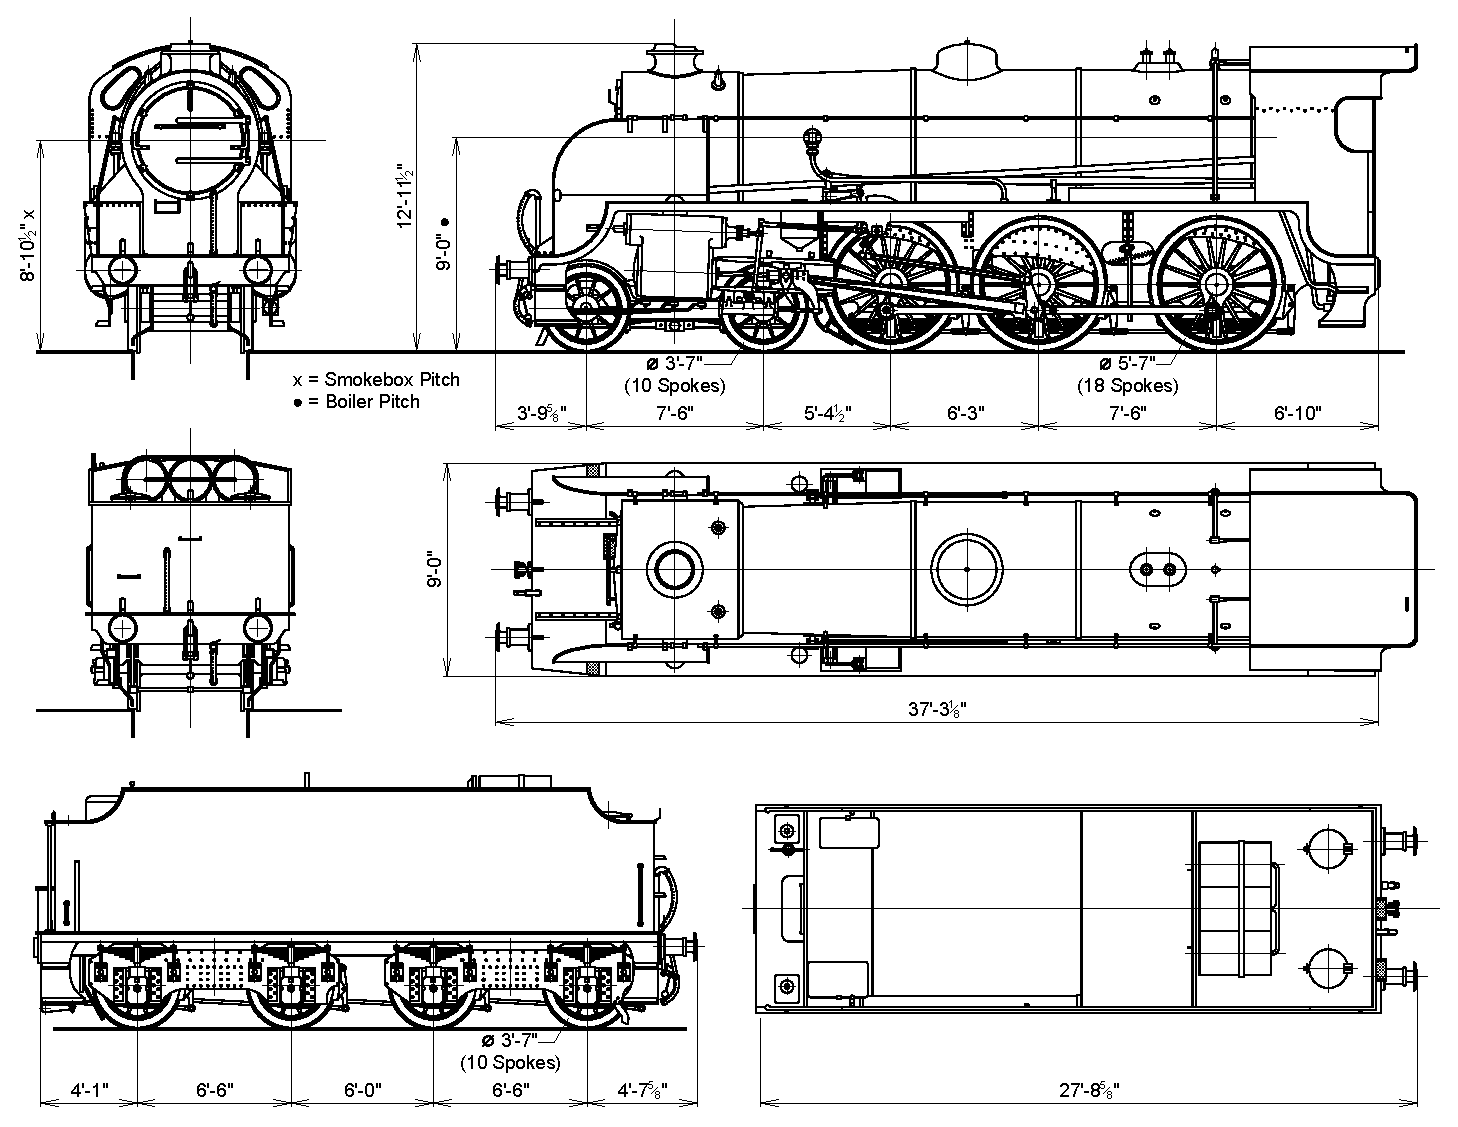
\includegraphics[angle=90,origin=c]{Images/SR_class_S15.eps}
}
\end{center}
\newpage

\pagestyle{headings}

To fully understand the unit buzz and its usage, we must go a little bit into technical
details. Although we support an arbitrary length and angular unit, there is one length
and one angular unit, from which all other units are derived. By no means preffering
any unit system, the base length unit was chosen as millimeter and the base angular
unit is degree (90 degrees to the right angle). And actually all dimensions stored in the
SteamCAD files are internally stored in milimeters. (No angles are stored in SteamCAD
files.)

So, if you want to add a new unit, just enter it into DUnits.ini, specify the unit
type (length or angle) and specify the unit ratio to the base unit. Only note one
irregularity - while when specifying the ratio for a length unit as 1 in = 25.4 mm,
the ratio for angular unit is reversed: 1 min = 1/60 deg. This is chosen for
convenience - not to be forced to enter numbers with unlimited decimal fraction.

Each unit has a name, an abbreviation, and also an alternate abbreviation. The reason
for two abbreviations, or two forms, or two unit symbols is simple. Some unit have
a symbol, which we would like to see on the printed output, but this symbol is not
common and does not appear on most of the keyboards. So it would be nice if we need
to enter the unit name or abbreviation, to enter it in another form, available
from most of the keyboards easily. An example of such a unit is degree. While we would
like to see the ``$^{\circ}$'' in the output, it is much more convenient to enter ``deg''
when specifying the unit while drawing.


\section{Entering Precise Values}
\special{pdf: out 2 << /Title (\thesection. Entering Precise Values) /Dest [ @thispage /FitH @ypos ] >>}

As we've seen in the section~\ref{sec:settings}, there are three default units
which can be set for the drawing. The default unit means that if you enter a value
into the edit box without any unit specification, the default unit is used for
the given context. However, you are not restricted on entering the values using
the default unit. If you want to enter a value in another unit than the default,
just specify any unit abbreviation with the value.

Example, you have millimeters as default unit, but you want to enter an imperial
dimension - just type 5in, or 5\primitiveQuote{} in the edit box.

And that's not all. The SteamCAD edit box also works as a primitive calculator.
So if you know the wheel diameter is 1856 mm, you don't need to divide it by two
to enter the circle with the correct radius. Just type 1856/2 in the edit box.

You also don't need to recalculate values to one unit. Just type ``10cm 8mm'' in the
edit box to get the length 18 mm exactly. This is quite simple, but putting
5\primitiveApostophe{}-3$\sfrac{2}{5}$\primitiveQuote{} would be more difficult. However,
in SteamCAD, you can just enter ``5\primitiveApostophe{}3+2/5\primitiveQuote''. But
please don't enter it as ``5\primitiveApostophe{} - 3+2/5\primitiveQuote''. SteamCAD
would interpret the hyphen symbol as minus in this case and would subtract
3$\sfrac{2}{5}$\primitiveQuote{} from 5\primitiveApostophe.

Also if you need to put 0.33333333333333333, just enter 1/3. If you need 0.66666\dots,
you can enter 2/3 or 1 - 1/3. And you get the fractional value with maximum accuracy.
SteamCAD also understands a predefined constant ``pi'', which is being interpreted
as $\pi$.


\section{Dimensioning and Labeling}
\special{pdf: out 2 << /Title (\thesection. Dimensioning and Labeling) /Dest [ @thispage /FitH @ypos ] >>}

A technical drawing has very little or no meaning without dimensions. So of course,
SteamCAD support dimensioning, however, SteamCAD does it in a way different from
other CAD systems. Most of CAD systems let you click three points and generate the
whole dimension including the label for you. Not so SteamCAD.

If you want to put a dimension in SteamCAD, you have to draw all the dimension
lines and supporting lines yourself, using standard primitives. As I spoke to
several engineers, this would be a nightmare for them. But there exists a reason
for doing it in this way - SteamCAD is focused on the presentation output, not
for creating an asset for manufacturing. So each SteamCAD product should be more
artistic work than engineering drawing. It means that the user needs full control
on how all the lines are placed.

So to enter a dimension, select any primitive, enter dimension mode by the ``D''
shortcut, and click two points on the line to place the dimension. As was mentioned,
you can select ANY primitive to place the dimension along, not only a line. If you
place a dimension on the line, SteamCAD will guess that the dimension will be
of length type. If the selected primitive is a circle, SteamCAD will guess that the
dimension will be angular. If the primitive is of any other type, SteamCAD will
have no guess and place three question marks as the label.

Once you insert a dimension, it is created with default arrows and if it is
distance or angle, also with default mask for that dimension. Double clicking the
dimension label, you can edit the dimension properties - the arrow types, sizes,
label font, label size, and the label content.

The label content is so called dimension mask. The mask can mix both plain text
and placeholders for substituting values. The placeholders can be marked either
by square brackets [] or by curly brackets \{\}. If the placeholder is marked
by square brackets, it means that the real world value will be substituted. If
the placeholder is marked bu curly brackets, the scaled values will be substituted.

The default mask for length label is [D:2], which means that real value in millimeters
with two decimal places will be substituted, and no dimension symbol will be placed
to the label. The defaul mask for angular dimension is [r:2]$^\circ$ which means
that angle in degrees with two decimal places will be substituted, followed by the
degree symbol.

If you want the label to represent paper length in milimeters without the unit
symbol, change it to \{D:2\}. If you don't specify the precision, it will be
printed with 6 decimal digits. If you specify the precision as zero (:0), it
will be printed without decimal places and separator.

You can also specify the precision as ``f''. In this case, the non integer part
will be printed as a fraction with denominator up to 64. So if you want to print
labels as on the SR class S15 example, specify the dimension mask as
[ft:0]\primitiveApostophe{}-[in:f]\primitiveQuote{}.

If it happens that SteamCAD does not want to format the label how you wish, you
can omit the placeholder and only put a plain text in the mask. In this case
it will be printed as it is, with two exceptions - if you want to print
5\primitiveApostophe{}-3$\sfrac{2}{5}$\primitiveQuote{}
put it as 5\primitiveApostophe{}-3\_2/5\primitiveQuote{}. And if you want to print
the symbol for diameter, put asterisk (*) at the begining of the mask (outside all
possible placeholders). If the mask starts with asterisk, it will be interpreted
as the diameter symbol (similar to \O).

Finally, note that it is possible to specify the default length and angular mask
in the document properties dialog.

You can also move and rotate the dimension labels using the standard Move and
Rotate commands. You can also use the dimensions for creating a standalone
labels. In this case, create a dummy line, put a dummy dimension on it. Set
the line thickness to a negative value, set the dimension arrows to none and
set the label content to a plain text.

\section{Saving and Opening Files}
\special{pdf: out 2 << /Title (\thesection. Saving and Opening Files) /Dest [ @thispage /FitH @ypos ] >>}

SteamCAD stores the files in its own binary format with extension .sdr. The files
should be transferable between Linux and Windows. There are fairly known commands
\textbf{New}, \textbf{Open}, \textbf{Save} and \textbf{Save as} which create,
read and write sdr files. Besides those, there are also \textbf{Save Selection\dots}
and \textbf{Include\dots} commands. The first one only saves the objects selected
in the current drawing to a new file. This is if you draw a steam engine with a
tender and you find that the tender migth be re-used for another locomotive class.
The \textbf{Include\dots} command will import an sdr file while keeping the drawing
opened. Those two commands somehow replace the missing clipboard.

\section{Exporting Files}\label{sec:export}
\special{pdf: out 2 << /Title (\thesection. Exporting Files) /Dest [ @thispage /FitH @ypos ] >>}

The sdr files only hold the drawing definition, they should not serve as the final
SteamCAD output. SteamCAD drawings are supposed to undergo some further processing
to get published or presented. That's why SteamCAD implements variety of export
formats.

The first one is \textbf{PDF} (portable drawing format) format. This is good if you
want to quickly review your drawing or if you want to print it. All PDF viewers should
implement printing.

Other two export formats are \textbf{PS} (postscript) and \textbf{EPS} (encapsulated
postscript). The first one can be sent directly to a postscript enabled printer.
The second one is intended to be included in larger documents. This manual is an
example of using EPS files. It is written in \LaTeX{} and the SteamCAD images were
included as EPS figures.

The fourth export format is \textbf{SVG} (scalable vector graphics), which is an xml
based text format natively supported by most of the web browsers. So such a file
is suitable for presenting its content on the web. Lot's of drawing programs,
such as Inkscape, also allow importing SVG files, so this format can be used for
further processing of the image.

The fifth format is \textbf{PNG} (portable network graphics), which is loselessly
compressed raster file. The SteamCAD graphics is exported with fixed resolution
600 dpi. The raster file can be further processed in an image manipulation
program, such a GIMP.

The last format is \textbf{DXF} (drawing exchange format). The implementation
of this format is quick and dirty, and it is not intended for serious work. However,
the format can be read by most of the CAD systems, so it might be possible to
import a SteamCAD drawing into another CAD, but it would certainly require lots
of manual adjustments, since DXF format philosophy is far away from the SteamCAD's
one.

\section{Patterned Lines Conflict Resolution}
\special{pdf: out 2 << /Title (\thesection. Patterned Lines Conflict Resolution) /Dest [ @thispage /FitH @ypos ] >>}

Drawing patterned lines used to have strong rules when the drawing were created
by hands. These rules were mostly relaxed with dawn of CADs, since it was too
difficult to implement them and too easy to live without them. Aestetics is simply
not something to bother about.

However, the printing quality is important for SteamCAD, so some of the rules
for placing patterned lines were implemented. Namely, when drawing patterned
lines, the author should avoid crossing lines at the voids. Since it is not always
possible, SteamCAD does not attempt to detect all such places automatically, but
it provides a tool called \textbf{Mark Conflicts} (with a shortcut ``Ctrl + F'')
to manually enter places which should be covered by the first element of the
line pattern. Please note the FIRST, it means that not the longest element, but the
first one in the definition will be attempted to cross the conflict point. So
it is advantageous to define the first element of a pattern as the longest one.

\begin{figure}[h]
\begin{center}
\includegraphics{Images/Conflicts.eps}
\end{center}
\end{figure}

The previous figure shows the difference when not specifying conflicts (left
image) and with conflicts at the center and circle boundary (right image).
As you can see, the line pattern is considered to be a ``rubber band'' and
can be stretched to fulfill the requirements.

You can unmark the conflict by clicking at the conflict position again
while in mark conflicts mode. Also when you mark as conflicted an end of
the line, only the half of the first element will be drawn at that position.
This can be used when creating a petterned line of several smoothly joined
curves. Such a join can be observed on the first class 6 locomotive, inside
the driver's cab.

\section{Rescale Images and Change Dimensions}
\special{pdf: out 2 << /Title (\thesection. Rescale Images and Change Dimensions) /Dest [ @thispage /FitH @ypos ] >>}

There are few more commands left, which we haven't discussed yet.
\begin{enumerate}
\item \textbf{Mesure distance} (``Alt + D'') - you can measure any distance
by clicking two consequent points. The distance and angle is reported on
the status bar in the default units and depending on the Paper units switch,
they are reported either in world default units, or paper default units.
\item \textbf{Tools \lar{} Rescale and Units} - this command can be used to
both change the default length and angular mask for the whole drawing and to
change the scale of the whole drawing. To change the mask can be useful if you
created a drawing at a given scale, say 1:87, all the dimensions are reported
in world distances, and you will find that for modelling purpose, it will be
better to know the scaled dimensions. After running the command, all dimensions
will be changed to paper units.

To rescale the whole drawing may be handy if you create the drawing say at
scale H0 (1:87) and later you find that a drawing at the scale TT (1:120) would
also be nice.
\item \textbf{Tools \lar{} Statistics} - this command displays a simple dialog box showing how
many elements and what primitive types are used in the drawing.
\end{enumerate}


